\documentclass[10pt,a4paper]{report}

% -------------------------------------------------
% Packages
% -------------------------------------------------
\usepackage[T1]{fontenc}
\usepackage[utf8]{inputenc}
\usepackage[swedish]{babel}
\usepackage{lmodern}

\usepackage[a4paper, margin=1.5cm]{geometry}

\usepackage{xcolor}
\usepackage{amsmath,amssymb}
\usepackage{array}
\usepackage{booktabs}
\usepackage{longtable}
\usepackage{graphicx}
\usepackage{float}
\usepackage{parskip}
\usepackage{enumitem}
\usepackage{listings}
\usepackage[most]{tcolorbox}
\usepackage{hyperref}
\usepackage{tikz}
\usetikzlibrary{trees}

% -------------------------------------------------
% Colors
% -------------------------------------------------
\definecolor{primary}{RGB}{30,58,138}
\definecolor{secondary}{RGB}{15,118,110}
\definecolor{accent}{RGB}{180,83,9}
\definecolor{codebg}{RGB}{248,250,252}
\definecolor{codeframe}{RGB}{203,213,225}

% -------------------------------------------------
% Python Listings
% -------------------------------------------------
\lstset{
  language=Python,
  backgroundcolor=\color{codebg},
  basicstyle=\ttfamily\small,
  keywordstyle=\color{primary}\bfseries,
  stringstyle=\color{secondary},
  commentstyle=\color{accent}\itshape,
  showstringspaces=false,
  breaklines=true,
  frame=single,
  rulecolor=\color{codeframe},
  numbers=left,
  numberstyle=\tiny,
  numbersep=5pt,
  tabsize=4
}

% -------------------------------------------------
% Boxes
% -------------------------------------------------
\newtcolorbox{conceptbox}[1]{
  colback=white,
  colframe=primary,
  fonttitle=\bfseries\color{white},
  title=#1,
  arc=2mm,
  boxrule=0.8pt
}

\newtcolorbox{intuitionbox}[1]{
  colback=codebg,
  colframe=secondary,
  fonttitle=\bfseries\color{white},
  title=#1,
  arc=2mm,
  boxrule=0.8pt
}

% -------------------------------------------------
\title{\Huge Formelblad: OOP i Python}
\author{Disa Degerholm}
\date{}

% -------------------------------------------------
\begin{document}

\maketitle

\tableofcontents

%%%%%%%%%%%%%%%%%%%%%%%%%%%%%%%%%%%%%%%%%%%%%%%%%%%%
\chapter{Object-Oriented Programming (OOP)}
%%%%%%%%%%%%%%%%%%%%%%%%%%%%%%%%%%%%%%%%%%%%%%%%%%%%

\section{Grundbegrepp}

\begin{conceptbox}{Viktiga Begrepp}
\begin{itemize}[leftmargin=*]
  \item \textbf{OOP}: \texttt{print(str)} kan ta in variabler med olika syntax. Funktion med specifika datatyper den tar in, t.ex. \texttt{write(filename)}.
  \item \textbf{Klass}: Regler (t.ex. \texttt{print}, \texttt{write}) -- regler med tom data. \texttt{def} skapar objekt (referenser/kopia).
  \item \textbf{Objekt}: Kopia av klass / exempel på klass -- regler med data (kopia + data).
  \item \textbf{Instans}: Ett specifikt objekt som man refererar till (t.ex. \texttt{mom}, \texttt{siblings}, \texttt{sibling}).
  \item \textbf{Attribut}: Variabler i objektet/klassen.
  \item \textbf{Metod}: Funktion som hör till klassen.
\end{itemize}
\end{conceptbox}

\begin{intuitionbox}{Intuition}
En klass är regler utan data.

Ett objekt är en kopia av klassen fylld med data.

En instans är det specifika objektet du syftar på.
\end{intuitionbox}

\section{Syntax för Klasser och Objekt}

\begin{lstlisting}
# Syntax for klasser
class Bilar: # Bor namnges med stor bokstav i borjan, ska vara ett substantiv (t.ex. Bilar)

    competition = "Formula 1" # Klassattribut, delad av alla objekt i klassen

    def __init__(self, age, arg2): # Instansattribut, unik for varje objekt genom att data laggs till
        self.age = age # Har skapas attribut/variabler (t.ex. alder, vikt)
        self.weight = arg2
    
    def varde(self): # Funktion/metod som beraknar bilens varde
        pengar = self.age * 1000 + self.weight * 500 # Obs: aven enkla funktioner som len() behovs laggas till sa de funkar pa din klass
        return pengar

    # Lagg till enkla funktioner vi vill ha
    def __str__(self): # __str__() ar en speciell metod som definierar hur objektet ska representeras som en strang
        return f"Bil med alder: {self.age}, vikt: {self.weight}, tavling: {Bilar.competition}"
    
    def __len__(self):
        pass
    
    def hoarse_happines(self):
        return self.age    2

# Syntax for att skapa ett objekt (instans) av klassen
objekt = Bilar(2, 800) # Objekt kan nu manipulera hela datan fran Bilar med hjalp av enkel punktnotation
objekt.attribut3 = 10 # Har kan man lagga till fler attribut, obs kan skrivas over
objekt.varde() # Har kan man anropa metoder som redan finns i klassen
objekt2 = Bilar(5, 1000) # Har skapas ett nytt objekt med annan data som en kopia
print(objekt2.age) # For att anvanda funktioner som redan finns pa objektet, kalla pa dess info/attribut

VolvoW80 = Bilar(2, 800)
volvo_pengar = VolvoW80.varde()
Hoarses = Bilar(7, 900)
\end{lstlisting}

%%%%%%%%%%%%%%%%%%%%%%%%%%%%%%%%%%%%%%%%%%%%%%%%%%%%
\chapter{Inkapsling och Arv}
%%%%%%%%%%%%%%%%%%%%%%%%%%%%%%%%%%%%%%%%%%%%%%%%%%%%

\section{Privata Attribut och Metoder}

\begin{lstlisting}
class Bil:
    def __init__(self, alder, vikt):
        self._alder = alder  # Privata attribut (bor inte andras utanfor klassen)
        self._vikt = vikt    # Privata attribut (bor inte andras utanfor klassen)

    def berakna_varde(self):
        return self._alder * 1000 + self._vikt * 500  # Publik metod som anvander privata attribut

min_bil = Bil(5, 1500) # Man kan manipulera med berakna_varde() men inte andra _alder eller _vikt direkt om man inte skrivs...
min_bil._alder = 10   # ...sa har, men det ar inte rekommenderat eftersom det bryter mot principen om inkapsling.
\end{lstlisting}

\section{Arv (Inheritance)}

\begin{itemize}[leftmargin=*]
  \item \textbf{Syfte}: Återanvända, lägga till eller ändra funktionalitet i befintliga klasser.
  \item \textbf{Termer}: \texttt{Basklass} / \texttt{Superklass} / \texttt{Parent class} (klassen man ärver från). \texttt{Subklass} / \texttt{Child class} (klassen som ärver).
  \item \textbf{Automatisk ärvning}: Metoder och klassattribut ärvs automatiskt. Instansattribut ärvs \textbf{inte} automatiskt om \texttt{\_\_init\_\_} definieras om i subklassen.
  \item \textbf{super()}: Används i subklassens konstruktor för att anropa basklassens konstruktor och ärva dess instansattribut.
\end{itemize}

\begin{lstlisting}
class A:
    class_integer = 10 # attribut som arvs av alla subklasser
    def __init__(self):
        self.vals = [5] # attribut som inte arvs av subklasser om __init__ definieras om
    def power_sum(self):
        return sum([i  2 for i in self.vals]) + A.class_integer # self.vals=[5] -> 5  2 + 10 = 35

class B(A): # B arver fran A
    def __init__(self, x, y): # (self, x, y) kommer fran input och inte forbestams
        self.vals = [x, y] # Definierar om instansattribut utan super()
    def print_result(self):
        print(self.power_sum()) # Anvander metod fran A

class C(A):
    def __init__(self, y):
        super().__init__() # Anropar A:s __init__ sa self.vals skapas!
        self.vals.append(y)

a = A()          # a.power_sum() -> 35
b = B(10, 20)    # b.power_sum() -> 510
c = C(10)        # c.vals -> [5, 10], c.power_sum() -> 135
\end{lstlisting}

\section{Klassdiagram \& Liskovs Substitutionsprincip}

\begin{itemize}[leftmargin=*]
  \item \textbf{Klassdiagram (UML)}: Visualiserar hur klasser hänger ihop oavsett tidpunkt (visar relationer mellan klasser som "is-a", medan om en klass inehåller ett objekt från en annan klass med \textbf{komposition}). Ett \textbf{objektdiagram} visar tillståndet i ett program vid en viss tidpunkt.
  \item \textbf{Liskovs substitutionsprincip}: Allt som gäller för en basklass ska också gälla för dess subklasser.
\end{itemize}

\section{Informationsfunktioner \& MRO}

\begin{itemize}[leftmargin=*]
  \item \textbf{isinstance(obj, Class)}: Returnerar \texttt{True} om \texttt{obj} är en instans av \texttt{Class} eller dess superklasser.
  \item \textbf{issubclass(Sub, Super)}: Returnerar \texttt{True} om klassen \texttt{Sub} ärver från \texttt{Super}.
  \item \textbf{MRO (Method Resolution Order)}: Den ordning Python söker efter metoder i arvskedjan. Kan visas med \texttt{Klass.mro()}.
  \item \textbf{Object}: Basklassen för alla typer och klasser i Python (\textit{"Everything is an object in Python"}).
\end{itemize}

\begin{lstlisting}
isinstance(a, A)      # True
isinstance(c, A)      # True (c arver fran A)
issubclass(B, A)      # True
issubclass(str, object)# True

print(B.mro()) # [__main__.B, __main__.A, object]
\end{lstlisting}

\section{Exempel: Geometriska Figurer (Arvs-kedja)}

Exemplet visar hur en basklass \texttt{Polygon} utökas och specialiseras av \texttt{Triangle}, \texttt{Rectangle} och \texttt{Square} med hjälp av metodöverlagring och \texttt{super()}.

\begin{lstlisting}
class Polygon:
    __name__ = "Polygon" # Hanterar endast symetriska former
    def __init__(self, n_sides, sides=None):
        self.n_sides = n_sides # Antal sidor (int) 
        self.sides = sides if sides else [1 for _ in range(n_sides)] # Lista med sidlangder (float)
        self.check_sides() # kallar pa check_sides() for att validera sidlangderna

    def check_sides(self):
        if not self.sides or not all(map(lambda x: x > 0, self.sides)):
            raise ValueError("Invalid side lengths")
        if self.n_sides != len(self.sides):
            raise ValueError("Wrong number of sides")

    def set_sides_from_input(self, n_unique_sides=None): # malet ar att kunna mata in t.ex. 2 unika sidor for en rektangel (dvs 2 sidor ar lika langa) och fa ut sides som [a, b, a, b] (dvs 4 sidor totalt)
        if not n_unique_sides: n_unique_sides = self.n_sides # Om inget valts: anta at alla sidor ar unika -> inlasning av lika manga unika langder som totalt antal sidor
        if self.n_sides % n_unique_sides != 0: # Om totala antalet sidor inte ar en multipel av unika sidor: fel
            raise ValueError("Total sides must be multiple of unique sides")
        unique = [float(input(f"Enter side {i+1}: ")) for i in range(n_unique_sides)] # las in en sida i taget for de n_unique_sides
        self.sides = unique * (self.n_sides // n_unique_sides) # retuernera antal sidor i en lista med de unika langderna upprepade sa at totala antalet sidor blir n_sides, e.x. [a, b] * 2 = [a, b, a, b] for en rektangel med 4 sidor 
        self.check_sides() # se sidor ar validerade

class Triangle(Polygon):
    __name__ = "Triangle"
    def __init__(self, sides=None):
        super().__init__(3, sides)

    def check_sides(self):
        a, b, c = sorted(self.sides)
        if not (c < a + b):
            raise ValueError(f"Shortest sides must be > longest in {self.__name__}") # Har betyder self.__name__ Triangle
        super().check_sides() # Har fortsatter checken mha gamla testerna

    def get_area(self):
        a, b, c = sorted(self.sides)
        s = (a + b + c) / 2
        return (s * (s - a) * (s - b) * (s - c))    0.5

class Rectangle(Polygon):
    __name__ = "Rectangle"
    def __init__(self, sides=None):
        super().__init__(4, sides)

    def check_sides(self):
        a, b, c, d = self.sides
        if not (a == c and b == d):
            raise ValueError(f"Opposite sides must be equal in {self.__name__}")
        super().check_sides()

    def get_area(self):
        return self.sides[0] * self.sides[1]

    def get_diagonal(self):
        return (self.sides[0]  2 + self.sides[1]  2)    0.5

class Square(Rectangle):
    __name__ = "Square"
    def __init__(self, sides=None):
        super().__init__(sides)

    def check_sides(self):
        a, b, c, d = self.sides
        if not (a == b == c == d):
            raise ValueError(f"All sides must be equal in {self.__name__}")
        super().check_sides()

    def get_corner_coordinates(self):
        s = self.sides[0] / 2
        return ((-s, -s), (-s, s), (s, s), (s, -s))
\end{lstlisting}

\begin{figure}[H]
    \centering
    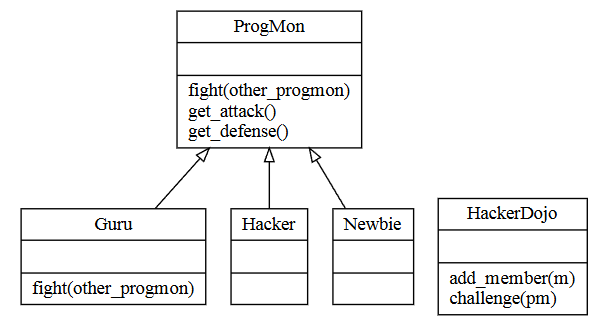
\includegraphics[width=0.9\textwidth]{Bilder/p1.png}
\end{figure}

%%%%%%%%%%%%%%%%%%%%%%%%%%%%%%%%%%%%%%%%%%%%%%%%%%%%
\chapter{Avancerad OOP: Operatorer \& Abstraktion}
%%%%%%%%%%%%%%%%%%%%%%%%%%%%%%%%%%%%%%%%%%%%%%%%%%%%

\section{Implementera Jämförelser (Operator Overloading)}

\begin{itemize}[leftmargin=*]
  \item Metoder som \texttt{\_\_lt\_\_} ($<$), \texttt{\_\_gt\_\_} ($>$) och \texttt{\_\_eq\_\_} ($==$) gör det möjligt att jämföra objekt.
  \item Om metoderna definieras i en basklass ärvs de automatiskt av alla subklasser.
\end{itemize}

\begin{lstlisting}
# Implementeras t.ex. i Triangle och Rectangle (Square arver automatiskt):
def __lt__(self, other):
    return self.get_area() < other.get_area()

def __gt__(self, other):
    return self.get_area() > other.get_area()

def __eq__(self, other):
    return self.get_area() == other.get_area()
\end{lstlisting}

\section{Exempel: Monster Go (Abstraktion \& Arv)}

\begin{itemize}[leftmargin=*]
  \item \textbf{Syfte}: Illustrera värdet av arv och abstraktion (dölja implementationsdetaljer via ett fast gränssnitt).
  \item \textbf{Privata attribut/metoder}: Inleds med \texttt{\_} (t.ex. \texttt{\_attack}) eller magiska metoder (\texttt{\_\_str\_\_}).
\end{itemize}

\begin{lstlisting}
class ProgMon:
    def __init__(self):
        self._attack = 0.0
        self._defense = 0.0
        self._caffeinated = False
        self._unit_testing = False

    def __str__(self):
        return "<ProgMon object>"

    def get_attack(self):
        return 2 * self._attack if self._caffeinated else self._attack

    def get_defense(self):
        return 2 * self._defense if self._unit_testing else self._defense

    def fight(self, other_progmon):
        if self.get_attack() > other_progmon.get_defense():
            return (True, False) # self vinner, return som tulp
        elif other_progmon.get_attack() > self.get_defense():
            return (False, True) # other vinner
        else:
            return (False, False) # Oavgjort

'''
Skapa monster: p1 = ProgMon() -> Andra status: p1._caffeinated = True -> p1.fight(p2) kors 
-> p1.get_attack() (dubblerad) jamfors mot p2.get_defense() -> returnerar resultat som 
tuppel: (True, False)
'''
\end{lstlisting}

\section{Subklasser \& Metodöverlagring (Overriding)}

\begin{itemize}[leftmargin=*]
  \item \textbf{Specialisering}: Subklasser sätter sina egna värden på skyddade attribut och kan skriva om metoder.
  \item \textbf{Metodöverlagring}: Om en subklass definierar om en metod (t.ex. \texttt{fight} i \texttt{Guru}) ändras beteendet utan att anropande kod behöver ändras.
\end{itemize}

\begin{lstlisting}
class Hacker(ProgMon):
    def __init__(self):
        super().__init__()
        self._attack = 0.5
        self._defense = 0.25
    def __str__(self):
        return "<Hacker A=" + str(self._attack) + ">" # print(Hacker()) -> <Hacker A=0.5>

class Newbie(ProgMon):
    def __init__(self):
        super().__init__()
        self._attack = 0.15
        self._defense = 0.1
    def __str__(self):
        return "<Newbie>"

class Guru(ProgMon):
    def __init__(self):
        super().__init__()
        self._attack = 1.0
        self._defense = 1.0

    # Overlagrar fight() med egna regler ("Don't win, don't lose")
    def fight(self, other_progmon):
        return (False, False)
\end{lstlisting}

\section{Aggregering \& Gränssnitt (HackerDojo)}

\begin{itemize}[leftmargin=*]
  \item \textbf{HackerDojo}: Innehåller en samling av \texttt{ProgMon}-objekt (aggregering).
  \item \textbf{Framtidssäkring via abstraktion}: \texttt{HackerDojo} behöver bara känna till gränssnittet (\texttt{.fight()}) – inte om monstrummet är en \texttt{Hacker}, \texttt{Newbie} eller \texttt{Guru}.
\end{itemize}

\begin{lstlisting}
class HackerDojo:
    def __init__(self):
        self._members = []

    def add_member(self, m):
        self._members.append(m)

    def challenge(self, pm):
        for monster in self._members:
            win, loose = pm.fight(monster)
            if loose: # dvs (nagot, True)
                return False # Forlorade mot minst en medlem
        return True # Klarade alla matcher utan forlust

# Anvandning:
dojo = HackerDojo()
dojo.add_member(Hacker())
dojo.add_member(Newbie())

g = Guru()
n = Newbie()
print(dojo.challenge(g)) # True (Guru forlorar aldrig pa grund av sin overlagrade fight-metod)
print(dojo.challenge(n)) # False
\end{lstlisting}

\begin{figure}[H]
    \centering
    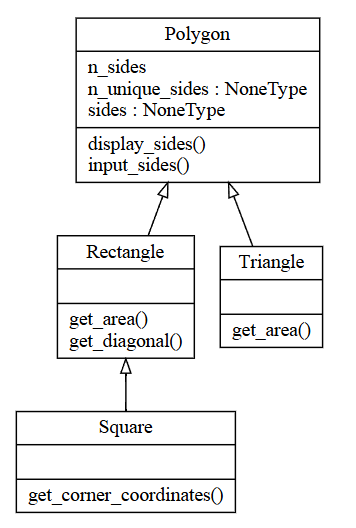
\includegraphics[width=0.3\textwidth]{Bilder/p2.png}
\end{figure}

\section{Olika typer av arv}
I förra kapitlet såg vi olika exempel på arv i Python. Olika former av arv har olika namn inom objektorientering:

\begin{enumerate}
    \item \textbf{Enkelt arv} (eng. \textit{single inheritance}): klass B ärver endast från klass A.
    \item \textbf{Mångnivåarv} (eng. \textit{multilevel inheritance}): klass B ärver från A och klass C ärver sen från klass B.
    \item \textbf{Hierarkiskt arv} (eng. \textit{hierarchical inheritance}): klass A är superklass till B, C, D\dots
    \item \textbf{Multipelt arv} (eng. \textit{multiple inheritance}): klass C ärver från \textit{både} A och B (men de ärver inte från varandra).
    \item \textbf{Hybridarv} (eng. \textit{hybrid inheritance}): en mix av två eller fler typer av arv.
\end{enumerate}

Vi såg även att man kan illustrera olika typer av arv med hjälp av klassdiagram. Förra kapitlet innehöll exempel på enkelt, mångnivå-, hierarkiskt och hybrid-arv, så vi ska nu titta på multipelt arv.

Det är inte alla programmeringsspråk som tillåter multipelt arv, men det gör Python. Betrakta följande exempel:

\begin{lstlisting}
class A:
    pass  # some code

class B:
    pass  # some more code

class C(A, B):
    pass  # even more code
\end{lstlisting}

Här har C alltså två superklasser, A och B, vilka inte ärver från varandra. Detta kan verka oskyldigt och man kan undra varför inte alla språk stödjer det. Men rent generellt är det lätt hänt att multipelt arv ger kaos på grund av så kallade \textbf{\textit{diamantproblem}}.

\subsection{Diamantproblem}
Betrakta följande kod:

\begin{lstlisting}
class A:
    def f(self):
        print("f of A called")

class B(A):
    def f(self):
        print("f of B called")

class C(A):
    def f(self):
        print("f of C called")

class D(B, C):
    pass

d = D()
d.f() # Ger f och B called och om C, B byter plats ges f och C called
\end{lstlisting}

Så utdata har nu ändrats då man ärver i en annan ordning! Denna typ av beroenden vill man helst inte behöva tänka på när man programmerar och därför tycker man att det är ett problem. 


\section{Algebraiska uttryck \& Rekursiva träd}

Genom att kombinera   klasser   och   rekursion   kan vi effektivt representera och manipulera hierarkisk data, som algebraiska uttryck och binära träd.

\subsection{Varför använda träd istället för strängar?}
Att representera algebraiska uttryck (t.ex. $x \cdot y + 7$) som vanliga strängar skapar problem vid utvärdering och variabelbyten. Strängar saknar strukturell information om t.ex. operatorprioritet och parenteser. 

Ett   binärt träd   löser detta genom att representera uttrycket i två dimensioner:
\begin{itemize}[leftmargin=*]
    \item   Noder:   Operatorer (\texttt{+}, \texttt{*}) som har vänster och höger underträd.
    \item   Löv:   Värden och variabler (\texttt{7}, \texttt{x}, \texttt{y}) utan underträd.
\end{itemize}

\begin{center}
\begin{tikzpicture}[level distance=0.8cm, sibling distance=1.2cm]
  \node {$+$}
    child { node {$*$}
      child { node {$x$} }
      child { node {$y$} }
    }
    child { node {$7$} };
\end{tikzpicture}
\quad \quad
\begin{tikzpicture}[level distance=0.8cm, sibling distance=1.2cm]
  \node {$*$}
    child { node {$x$} }
    child { node {$+$}
      child { node {$y$} }
      child { node {$7$} }
    };
\end{tikzpicture}
\end{center}

\subsection{Implementering med operatorprioritet (Precedence)}
För att skriva ut uttrycken korrekt med parenteser tilldelas varje operator ett prioritetsvärde (\texttt{prec}). Om ett underträd har lägre prioritet än sin förälder omsluts det med parenteser.

\begin{lstlisting}[language=Python]
class Expr: # star for Expression
    prec = 1000  # prec star for precedence, har hog

class Constant(Expr):
    def __init__(self, value):
        self._value = value
    def __str__(self):
        return str(self._value)

class Var(Expr):
    def __init__(self, name):
        self._name = name
    def __str__(self):
        return self._name

class BinOp(Expr):
    def __init__(self, left, right):
        self._left = left
        self._right = right

def parens(p1, p2, s): # parens star for parenteser
    return f"({s})" if p1 < p2 else s # p1 star for prioritet for foralder, p2 for prioritet for barn
    # Ex man vill satta parantes pa plus

class Plus(BinOp):
    prec = 1
    def __str__(self):
        s1 = parens(self._left.prec, self.prec, str(self._left))
        s2 = parens(self._right.prec, self.prec, str(self._right))
        return f"{s1} + {s2}"
# bygger en textstrang av tva uttryck genom att kontrollera om vanster- och hogerledet
# behover omges av parenteser utifran deras prioritetsvarden (prec).

class Times(BinOp):
    prec = 2
    def __str__(self):
        s1 = parens(self._left.prec, self.prec, str(self._left))
        s2 = parens(self._right.prec, self.prec, str(self._right))
        return f"{s1} * {s2}" 

# Exempel pa anrop och automatisk parenteshantering (lases fran hoger till vanster):
print(Plus(Times(Var("x"), Var("y")), Constant(7)))  # Out: x * y + 7
print(Times(Var("x"), Plus(Var("y"), Constant(7))))  # Out: x * (y + 7)
\end{lstlisting}


\section{Generella Binära Träd}

Mönstret ovan kan generaliseras till godtyckliga binära träd med rekursiva metoder för databearbetning.

\begin{itemize}[leftmargin=*]
    \item \texttt{\_\_str\_\_()}: Formaterar trädet rekursivt som en sträng.
    \item \texttt{member(x)}: Söker rekursivt i trädet efter värdet \texttt{x}.
    \item \texttt{map\_tree(f)}: Högre ordningens funktion som applicerar funktionen \texttt{f} på varje nod/löv.
    \item \texttt{linearize()}: Gör om trädstrukturen till en platt lista (in-order).
\end{itemize}

\begin{lstlisting}[language=Python]
class BinTree:
    pass

class Branch(BinTree):
    def __init__(self, node, left, right):
        self._node = node
        self._left = left
        self._right = right

    def __str__(self):
        return f"({self._node},{self._left},{self._right})"

    def member(self, x):
        return self._node == x or self._left.member(x) or self._right.member(x)

    def map_tree(self, f):
        return Branch(f(self._node), self._left.map_tree(f), self._right.map_tree(f))

    def linearize(self):
        return self._left.linearize() + [self._node] + self._right.linearize()

class Leaf(BinTree):
    def __init__(self, val):
        self._val = val

    def __str__(self):
        return f"({self._val})"

    def member(self, x):
        return self._val == x

    def map_tree(self, f):
        return Leaf(f(self._val))

    def linearize(self):
        return [self._val]

# Test och korning
t = Branch(-32, Leaf(2), Branch(1, Branch(23, Leaf(4), Leaf(-2)), Leaf(12)))

print(t)                      # (-32,(2),(1,(23,(4),(-2)),(12)))
print(t.member(12))           # True
print(t.map_tree(lambda x: x  2)) # Kvadrat pa alla element
print(t.linearize())          # [2, -32, 4, 23, -2, 1, 12]
\end{lstlisting}

\begin{figure}[H]
    \centering
    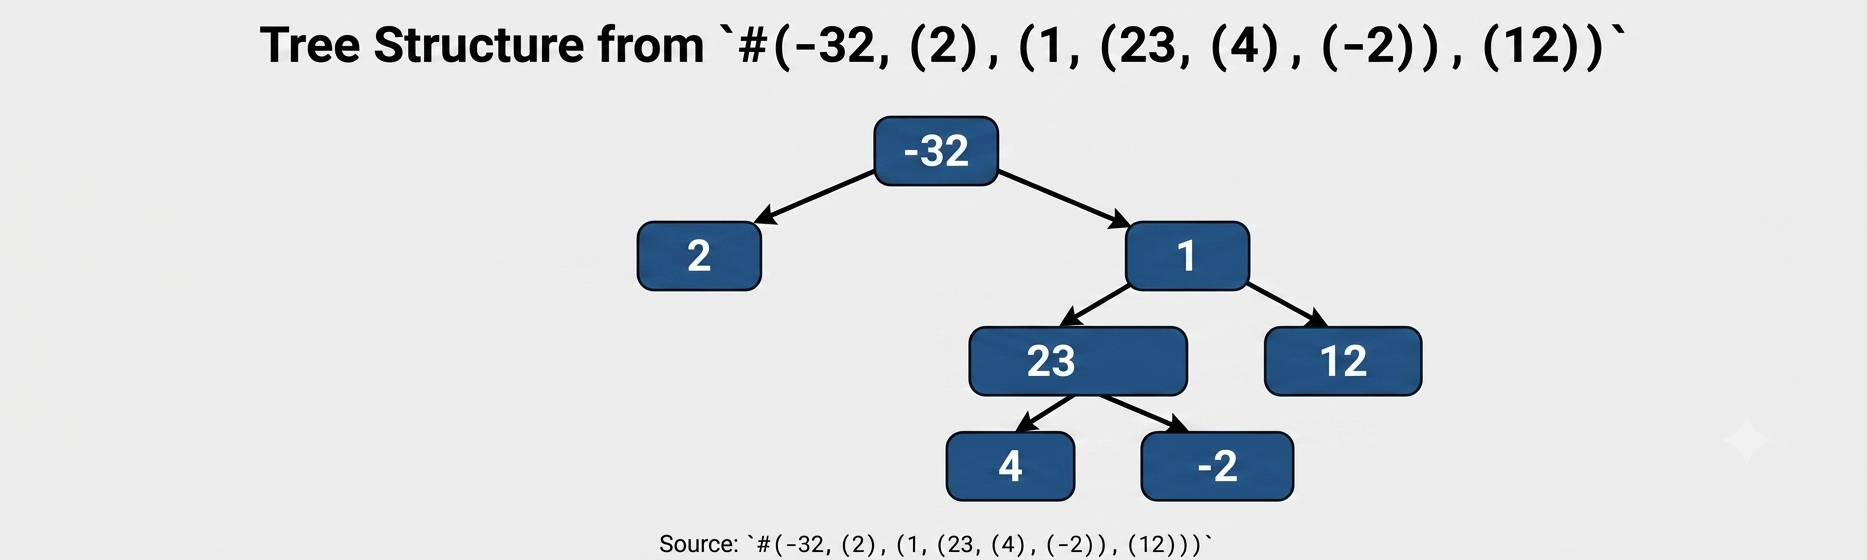
\includegraphics[width=0.9\textwidth]{Bilder/p3.png}
\end{figure}

%%%%%%%%%%%%%%%%%%%%%%%%%%%%%%%%%%%%%%%%%%%%%%%%%%%%
\chapter{Defensiv Programering}
%%%%%%%%%%%%%%%%%%%%%%%%%%%%%%%%%%%%%%%%%%%%%%%%%%%%

\section{Defensiv programmering \& Testning}

Defensiv programmering handlar om att koda sina antaganden för att upptäcka fel tidigt, nära felkällan, och undvika långvarig felsökning.

\subsection{Assert (Antaganden i koden)}
\begin{itemize}[leftmargin=*]
    \item \textbf{Syfte:} Verifiera att internt tillstånd är korrekt under utveckling/felsökning.
    \item \textbf{Beteende:} Om villkoret är falskt kastar Python ett \texttt{AssertionError}.
    \item \textbf{Syntax:} \texttt{assert condition,  ["Optional error message"]}
    \item \textbf{Optimeringsflagga:} Körs programmet med \texttt{python -O script.py} inaktiveras alla \texttt{assert}.
\end{itemize}

\begin{lstlisting}[language=Python]
def divide(x, y):
    # Ensure denominator is non-zero
    assert y != 0, "Second argument cannot be 0 when dividing"
    return x / y
\end{lstlisting}

\subsubsection{Klassificering av villkor}
\begin{itemize}[leftmargin=*]
    \item \textbf{Förvillkor (Preconditions):} Krav på indata som måste gälla när en funktion anropas.
    \item \textbf{Eftervillkor (Postconditions):} Krav på utdata/resultat när en funktion returnerar.
    \item \textbf{Invarianter (Loop/Class Invariants):} Tillstånd som alltid måste hålla under körning eller mellan metodanrop.
\end{itemize}

\begin{lstlisting}[language=Python]
class MyDB: # DB stands for database
    def __init__(self):
        self._id2name_map = {}
        self._name2id_map = {}

    def add(self, id, name):
        # Preconditions: Type checks
        assert isinstance(id, int), "ID must be integer" # isinstance() returns True or False
        assert isinstance(name, str), "Name must be string"
        self._name2id_map[name] = id
        self._id2name_map[id] = name

    def by_name(self, name):
        id = self._name2id_map[name]
        # Invariant check: Bi-directional map must match
        assert self._id2name_map[id] == name # checks if the id maps back to the same name
        return id
\end{lstlisting}

---

\subsection{Automatiserad testning}
För att säkerställa att ny funktionalitet inte förstör befintlig kod (\textit{regression testing}) används automatiserade tester.

\subsubsection{Enhetstester med \texttt{unittest}}
\begin{itemize}[leftmargin=*]
    \item \textbf{Struktur:} Tester grupperas som metoder i en klass som ärver från \texttt{unittest.TestCase}.
    \item \textbf{Assertion-metoder:} Använder specifika tester som \texttt{self.assertEqual(a, b)}, \texttt{self.assertTrue(x)}, etc.
    \item \textbf{Körning:} Startas med \texttt{unittest.main()} och om allt går rätt står "Ran X tests in Y s " och " OK" i terminalen.
\end{itemize}

\begin{lstlisting}[language=Python]
import unittest

class TestPolynomialOperations(unittest.TestCase):
    def test_addition(self):
        # Verify that adding polynomials is symmetric
        p = [2, 0, 1]
        q = [-2, 1, 0, 1]
        self.assertEqual(add_poly(p, q), add_poly(q, p), "Function should be symmetric")

    def test_evaluation(self):
        # Verify polynomial evaluation at x=0
        p = [2, 0, 1]
        self.assertEqual(eval_poly(p, 0), 2, "Should evaluate to constant term")

if __name__ == '__main__':
    unittest.main() # Run all defined test methods
\end{lstlisting}

\subsubsection{Slumptestning (Property-Based Testing)}
Istället för att skriva specifika testfall för hand definieras generella egenskaper (specifikationer) som koden måste uppfylla. Bibliotek som \texttt{hypothesis} genererar automatiskt slumpmässig indata för att hitta gränsfall där koden fallerar.

\end{document}